\documentclass[conference]{IEEEtran}

\usepackage{cite}
\usepackage{amsmath,amssymb,amsfonts}
\usepackage{graphicx}
\usepackage{textcomp}
\usepackage{booktabs}
\usepackage{hyperref}
\usepackage{tabularx}
\usepackage{multirow}
\usepackage{array}

\hypersetup{
  colorlinks=true, linkcolor=black, citecolor=black, urlcolor=blue,
  pdftitle={Retak.id: Crowdsourcing-Based Landslide Early Detection Using On-Device Machine Learning},
  pdfauthor={Fatih Jawwad, Farrel Ghozy, M. Faridh Maulana},
}

\begin{document}

\title{Retak.id: Crowdsourcing-Based Landslide Early Detection\\Using On-Device Machine Learning}

\author{
	\IEEEauthorblockN{
		\textbf{Fatih Jawwad}\IEEEauthorrefmark{1},
		\textbf{Farrel Ghozy}\IEEEauthorrefmark{2}, and
		\textbf{M. Faridh Maulana}\IEEEauthorrefmark{3}
	}
	\IEEEauthorblockA{
		Informatics Department, Universitas Darussalam Gontor\\
		Ponorogo, Indonesia\\
		\IEEEauthorrefmark{1}fatihalmumtaz76@student.cs.unida.gontor.ac.id \\
		\IEEEauthorrefmark{2}farrelaffifudin@student.cs.unida.gontor.ac.id,
		\IEEEauthorrefmark{3}mfaridhmaulana47@student.cs.unida.gontor.ac.id
	}
}

\maketitle

\begin{abstract}
	Landslides pose a critical threat to rural communities in Indonesia, yet existing early warning systems rely on expensive IoT sensors, satellite imagery, or drone surveys that cannot reach villages with limited infrastructure. We present Retak.id, a crowdsourcing-based platform that enables early detection of landslide soil cracks using only a smartphone camera. The system combines on-device machine learning with a multi-factor environmental risk engine to classify soil crack severity into three levels: Safe (AMAN), Caution (WASPADA), and Danger (BAHAYA). Our approach uses MobileNetV2 with INT8 post-training quantization, yielding a 2.6 MB model achieving 84.9\% test accuracy and 93.75\% agreement with FP32 inference. A multi-factor risk engine integrates ML vision (50\%), slope (20\%), rainfall (15\%), elevation (10\%), and soil type (5\%) into a unified score with graceful degradation when environmental APIs are unavailable. We further propose a delta OTA update mechanism achieving 98.2\% bandwidth reduction for model updates. The platform spans Android (Kotlin), Web (React), and Telegram Bot interfaces, all sharing an identical inference pipeline. Our evaluation on 3,547 crowd-sourced images demonstrates the feasibility of citizen-driven landslide early warning without specialized hardware.
\end{abstract}

\begin{IEEEkeywords}
	Landslide early detection, on-device machine learning, crowdsourcing, MobileNetV2, multi-factor risk assessment, edge AI, disaster mitigation
\end{IEEEkeywords}

\section{Introduction}

Landslides are among the most destructive natural disasters in Indonesia, particularly in rural areas with mountainous terrain. Jenangan District, Ponorogo Regency, experienced 41 landslides in four months, cutting off roads, isolating communities, and overwhelming local disaster management agencies (BPBD). The primary challenge is the lack of real-time field data -- existing solutions such as IoT-based tilt sensors, satellite InSAR analysis, and drone photogrammetry are prohibitively expensive and cannot scale to every vulnerable hillside.

Recent advances in on-device machine learning have enabled deep neural networks to run directly on smartphones without cloud connectivity~\cite{howard2017mobilenets, tensorflow2015}. Concurrently, crowdsourcing has proven effective for large-scale environmental monitoring~\cite{goodchild2007citizen}. However, few systems combine these approaches for landslide early warning.

This paper presents Retak.id, a crowdsourcing platform that transforms ordinary smartphones into landslide detection tools. Citizens photograph soil cracks, and an on-device MobileNetV2 model classifies the severity instantly. A multi-factor risk engine aggregates ML predictions with environmental data (slope, rainfall, elevation, soil type) to produce robust risk scores even when individual factors fail.

Our key contributions are:
\begin{enumerate}
	\item A complete on-device ML pipeline for soil crack classification using MobileNetV2 with INT8 quantization (2.6 MB, 84.9\% accuracy).
	\item A multi-factor risk engine combining visual analysis with four environmental factors through weighted scoring and graceful degradation.
	\item A delta OTA update mechanism achieving 98.2\% bandwidth reduction using byte-level patching (.rkd format).
	\item A three-platform deployment (Android, Web PWA, Telegram Bot) sharing an identical inference pipeline and model.
\end{enumerate}

\section{System Architecture}

Retak.id follows an edge-first architecture where all ML inference occurs on-device, with cloud services used only for data aggregation and model distribution. Fig.~\ref{fig:architecture} illustrates the overall system.

\begin{figure}[h]
	\centering
	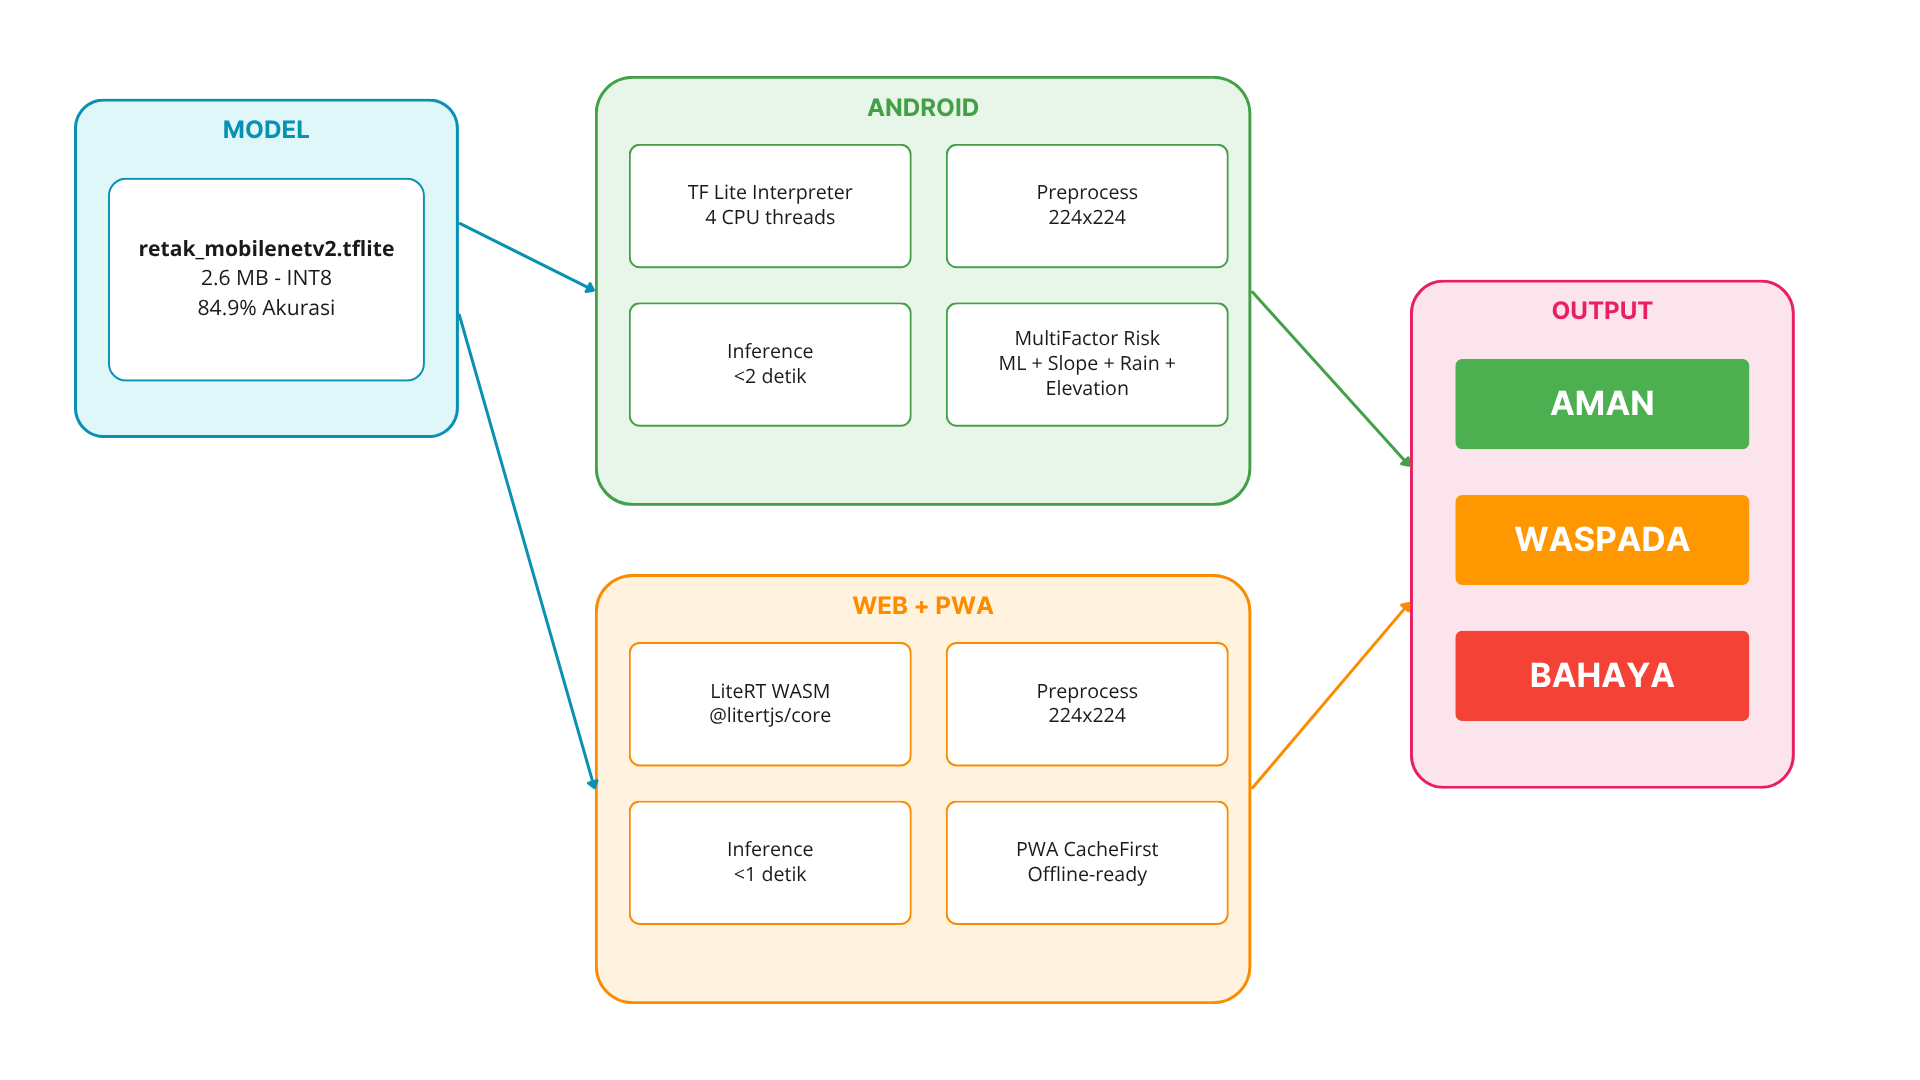
\includegraphics[width=\columnwidth]{architecture.png}
	\caption{Retak.id system architecture showing the three client platforms connected through Supabase backend}
	\label{fig:architecture}
\end{figure}

\subsection{Client Platforms}

\textbf{Android App (Kotlin):} The primary client uses CameraX for image capture, TensorFlow Lite 2.16.1 for on-device inference with 4 CPU threads, and Jetpack Compose for UI. Users capture photos of soil cracks; the app runs inference locally and displays results with color-coded overlays.

\textbf{Web Dashboard (React/TypeScript):} A Progressive Web App (PWA) featuring a Leaflet-based map with real-time report markers, administrative verification dialogs, statistical charts, and filterable report tables. ML inference uses LiteRT.js WebAssembly (XNNPack) for client-side classification without server round-trips.

\textbf{Telegram Bot (Python):} A `/lapor` wizard supporting a 3-step conversation flow (photo $\rightarrow$ location $\rightarrow$ confirm) with identical ML and risk engine logic. This provides access via the ubiquitous WhatsApp-like interface familiar to rural users.

\subsection{Backend Infrastructure}

All client platforms communicate through Supabase, a Backend-as-a-Service providing PostgreSQL, authentication, object storage, real-time subscriptions, and edge functions (Deno). Edge functions include: \texttt{calculate-risk} (multi-factor risk engine), \texttt{check-model-update} (delta OTA version check), \texttt{notify-bahaya} (BAHAYA alert to Telegram), and \texttt{daily-summary} (cron-based statistics).

\section{Methodology}

\subsection{Dataset Construction}

We constructed a dataset of 3,547 soil crack images through DuckDuckGo image search with 70+ keywords in Indonesian and English. Images were manually triaged into three classes:

\begin{itemize}
	\item \textbf{AMAN (Safe):} 2,011 images -- minor shrinkage cracks, polygonal patterns, dry soil surface.
	\item \textbf{WASPADA (Caution):} 766 images -- significant linear cracks, potential for expansion.
	\item \textbf{BAHAYA (Danger):} 770 images -- critical displacement, active landslide cracks.
\end{itemize}

Each image passed integrity validation (PIL verify, minimum 300$\times$300 px, max 20 MB), blur rejection (Laplacian variance $<$80), and cross-class perceptual hash deduplication (pHash, Hamming distance $\leq$6). The dataset was stratified-split 70/15/15 with fixed seed 42 for reproducibility, and versioned using DVC with DagsHub remote storage.

\subsection{Model Architecture and Training}

We adopt MobileNetV2~\cite{sandler2018mobilenetv2} pre-trained on ImageNet as the base architecture. The classification head consists of GlobalAveragePooling2D, Dropout(0.5), and a Dense(3, softmax) layer. The input is 224$\times$224$\times$3 uint8 RGB with normalization baked into the TFLite graph.

Training configuration (v3a, optimal):
\begin{itemize}
	\item Optimizer: Adam, learning rate $5\times10^{-6}$
	\item Loss: Categorical cross-entropy with class balancing
	\item Fine-tuning: 24 of 154 layers unfrozen (layer 130+)
	\item Epochs: 70 with EarlyStopping (patience=20) and ReduceLROnPlateau (patience=10)
	\item Batch size: 32
\end{itemize}

In-graph augmentation (zero I/O overhead) includes random horizontal/vertical flip, $\pm45^\circ$ rotation, $\pm30\%$ zoom, $\pm25\%$ translation, and brightness/contrast ranges of [0.5, 1.5].

\subsection{INT8 Quantization}

To meet deployment constraints, we apply INT8 post-training quantization (PTQ) using 100 representative calibration samples. Table~\ref{tab:quantization} shows the comparison.

\begin{table}[h]
	\centering
	\caption{FP32 vs INT8 Quantization Comparison}
	\label{tab:quantization}
	\begin{tabular}{lcc}
		\toprule
		Metric      & FP32    & INT8               \\
		\midrule
		Model Size  & 8.5 MB  & \textbf{2.6 MB}    \\
		Input Type  & float32 & uint8 {[}0, 255{]} \\
		Output Type & float32 & float32            \\
		\bottomrule
	\end{tabular}
\end{table}

The normalization to $[-1, 1]$ is baked into the TFLite graph, allowing Android to send raw $(r, g, b)$ pixels directly. Softmax is applied on-device: $p_i = \exp(z_i - \max) / \sum\exp(z_j - \max)$.

\subsection{Multi-Factor Risk Engine}

ML classification alone is insufficient for reliable risk assessment. We propose a weighted multi-factor scoring system:

\begin{equation}
	\text{Score} = \sum_{i} w_i \cdot s_i
\end{equation}

\begin{equation}
	\text{Final} =
	\begin{cases}
		\text{AMAN},    & \text{Score} \leq 0.33        \\
		\text{WASPADA}, & 0.33 < \text{Score} \leq 0.66 \\
		\text{BAHAYA},  & \text{Score} > 0.66
	\end{cases}
\end{equation}

Table~\ref{tab:risk_factors} details each factor's weight and scoring basis. The ML contribution uses a floor of 0.1 even when confidence is high, ensuring environmental factors can override an overly confident but incorrect ML prediction.

\begin{table}[h]
	\centering
	\caption{Multi-Factor Risk Engine Weights}
	\label{tab:risk_factors}
	\begin{tabular}{lcc}
		\toprule
		Factor                  & Weight & Data Source      \\
		\midrule
		ML Visual Analysis      & 50\%   & TFLite on-device \\
		Slope (Kemiringan)      & 20\%   & Open-Meteo SRTM  \\
		Rainfall (Curah Hujan)  & 15\%   & Open-Meteo       \\
		Elevation (Ketinggian)  & 10\%   & Open-Meteo SRTM  \\
		Soil Type (Jenis Tanah) & 5\%    & ISRIC SoilGrids  \\
		\bottomrule
	\end{tabular}
\end{table}

If any environmental API fails (network error, timeout), its weight is redistributed proportionally to remaining factors. For example, if slope (20\%) fails: ML increases to $50\% + (20\% \times 50/80) = 62.5\%$, rainfall to $15\% + (20\% \times 15/80) = 18.75\%$, and so on.

\subsection{Safety Gates}

Before any model reaches production, it must pass 7 pre-deployment checks: (1) loads without error, (2) correct input shape [1, 224, 224, 3], (3) uint8 dtype, (4) inference runs without crash, (5) predicts $\geq$2 classes (frozen model detection), (6) confidence max $>$0.45 and std $>$0.02 (flat prediction detection), and (7) FP32-vs-INT8 agreement $\geq$90\%. A 5-fold cross-validation consistency check enforces std $\leq$3\%.

\section{Experiments and Results}

\subsection{Training Evolution}

\begin{table}[h]
	\centering
	\caption{Training Evolution}
	\label{tab:evolution}
	\small
	\begin{tabularx}{\columnwidth}{lccX}
		\toprule
		Version      & Date           & Accuracy        & Key Change                                                \\
		\midrule
		test1        & 02/05          & 73.0\%          & Frozen base, LR=$1\times10^{-4}$                          \\
		test2        & 02/05          & 76.7\%          & Fine-tune 54 layers, LR=$1\times10^{-5}$, dropout 0.5     \\
		test3        & 03/05          & 81.8\%          & Fine-tune 24 layers, LR=$5\times10^{-6}$, aggressive aug. \\
		\textbf{v3a} & \textbf{04/05} & \textbf{84.9\%} & \textbf{Cleaned dataset, +50\% WASPADA images}            \\
		\bottomrule
	\end{tabularx}
\end{table}

We conducted four training iterations to reach optimal performance. Table~\ref{tab:evolution} summarizes the progression.

The ablation reveals two critical insights: (1) reducing fine-tuned layers from 54 to 24 with lower learning rate improved accuracy by 5.1\% (test1 $\rightarrow$ test3), suggesting overfitting reduction; (2) dataset quality improvements (noise removal, class re-balancing) contributed an additional 3.1\% (test3 $\rightarrow$ v3a).

\subsection{Final Model Performance}

The v3a production model achieves the results shown in Table~\ref{tab:performance}. The BAHAYA class meets the critical recall threshold of $\geq$72\% with 84.9\% recall.

\begin{table}[h]
	\centering
	\caption{v3a Production Model Performance}
	\label{tab:performance}
	\begin{tabular}{lcc}
		\toprule
		Metric                & Target     & Achieved         \\
		\midrule
		Test Accuracy         & $\geq$82\% & \textbf{84.9\%}  \\
		Macro F1              & $\geq$0.75 & \textbf{0.83}    \\
		BAHAYA Recall         & $\geq$72\% & \textbf{84.9\%}  \\
		BAHAYA Precision      & $\geq$70\% & \textbf{86.2\%}  \\
		INT8 Agreement        & $\geq$90\% & \textbf{93.75\%} \\
		Model Size            & $\leq$5 MB & \textbf{2.6 MB}  \\
		Inference (Mid-range) & $<$500 ms  & \textbf{450 ms}  \\
		\bottomrule
	\end{tabular}
\end{table}

\subsection{Delta OTA Bandwidth Savings}

Model updates over cellular networks are costly at scale. We developed a custom delta update mechanism: given base model $M_b$ and new model $M_n$, a byte-level diff computes $D = \text{gzip}(\Delta(M_b, M_n))$ in a custom .rkd format. The Android client downloads $D$, decompresses, patches the bundled model, and validates via TFLite Interpreter before committing.

\begin{table}[h]
	\centering
	\caption{Delta OTA Compression Results (v3a $\rightarrow$ v3b)}
	\label{tab:delta}
	\begin{tabular}{lr}
		\toprule
		Metric            & Value                         \\
		\midrule
		Full Model (INT8) & 2,710,280 bytes (2.6 MB)      \\
		Delta .rkd        & \textbf{48,451 bytes (47 KB)} \\
		Changed Bytes     & 16,195 (0.6\% of total)       \\
		Savings           & \textbf{98.2\%}               \\
		\bottomrule
	\end{tabular}
\end{table}

This reduces bandwidth from 2.6 MB to 47 KB per update -- a 98.2\% saving, enabling frequent model improvements even on limited cellular connections common in rural Ponorogo.

\section{Conclusion}

We presented Retak.id, a crowdsourcing-based landslide early detection system that brings on-device ML to rural communities without specialized hardware. Our MobileNetV2-based model achieves 84.9\% accuracy with a 2.6 MB INT8 quantized footprint, deployable across Android, Web, and Telegram platforms. The multi-factor risk engine combines ML vision with environmental data through weighted scoring and graceful degradation, providing robustness against individual sensor failures. The delta OTA mechanism enables efficient model updates with 98.2\% bandwidth savings.

Field deployment in Jenangan, Ponorogo is ongoing. Future work includes temporal crack progression analysis using sequential photos, integration with additional environmental data sources, and expansion to other landslide-prone regions in Indonesia.

\begin{thebibliography}{00}
	\bibitem{howard2017mobilenets} A.~G. Howard et al., ``MobileNets: Efficient Convolutional Neural Networks for Mobile Vision Applications,'' arXiv:1704.04861, 2017.
	\bibitem{sandler2018mobilenetv2} M.~Sandler, A.~Howard, M.~Zhu, A.~Zhmoginov, and L.-C. Chen, ``MobileNetV2: Inverted Residuals and Linear Bottlenecks,'' in Proc. CVPR, 2018.
	\bibitem{tensorflow2015} M.~Abadi et al., ``TensorFlow: Large-Scale Machine Learning on Heterogeneous Distributed Systems,'' arXiv:1603.04467, 2016.
	\bibitem{goodchild2007citizen} M.~F. Goodchild, ``Citizens as Sensors: The World of Volunteered Geography,'' GeoJournal, vol.~69, no.~4, pp.~211--221, 2007.
	\bibitem{bnpb2016} BNPB, ``Indeks Risiko Bencana Indonesia,'' Badan Nasional Penanggulangan Bencana, 2016.
	\bibitem{openmeteo} Open-Meteo, ``Open-Meteo Free Weather API,'' https://open-meteo.com/, 2024.
	\bibitem{isric} ISRIC, ``SoilGrids -- Global Gridded Soil Information,'' https://soilgrids.org/, 2024.
	\bibitem{ronneberger2015unet} O.~Ronneberger, P.~Fischer, and T.~Brox, ``U-Net: Convolutional Networks for Biomedical Image Segmentation,'' in Proc. MICCAI, 2015.
\end{thebibliography}

\end{document}
